%!TEX program = xelatex
	% Above tells TeX compiler to use xelatex. Necessary because can't manually set due to working in SublimeText and using LaTeXTools.

\documentclass[14pt, aspectratio=169, svgnames, xetex, rgb]{beamer}
	% 14pt: Increase base text size to make reading easier (important for math eqns)
	% aspectratio=169: Gives aspect ratio of 16:9 for better screen use and matching most commonly used aspect ratios. (Arguable that 1610 would be better, but the die is cast.)
	% svgnames: This one is a little surprising. It's not actually a Beamer option, it's an option for the 'xcolor' package. However, since Beamer loads that package on start, this option needs to be given now to be passed down to 'xcolor'. If you try to give the option to 'xcolor' (below), it will throw error warnings.
				% See note about 'svgnames' under 'xcolor' for usage regarding GLE.
	% xetex: Another 'xcolor' option like 'svgnames' is. This is perhaps totally unnecessary, but this sets the color driver. Since compiling is done with xelatex, it seemed like 'xetex' was the best choice.
	% rgb: Another 'xcolor' option like 'svgnames' is. This is perhaps totally unnecessary, but this chooses the target color model. Since all output is designed for monitor display, this seems like the best choice.


\usetheme[nooffset, noslidenumbers, blockbg]{m}
	% Theme showed by 'm' is "mtheme". It is a non-standard Beamer theme.
		% Theme was made by Matthias Vogelgesang. Thanks to him and other contributers.
		% Can find theme on GitHub: https://github.com/matze/mtheme
	% nooffset: Prevents mtheme from adding \vspace{2em} vertical offset at top of slides
	% noslidenumbers: Omits slide numbers on all slides

\usefonttheme{dailyplanet}
		% Self-devolped modification of font theme for Metropolis. Likely to change names in a future version. If you're trying to compile this in the future and it breaks, take a look in the docs for 'metropolis' / 'mtheme' theme style for Beamer. Look for alternate font themes. You'll want the one that mainly uses Fira Sans Book. Have fun finding it! :-D

	\setbeamertemplate{blocks}[rounded][shadow=true]
	% This rounds blocks and gives a dropshadow to blocks.
		% Note the slightly odd presentation of options here. This has to be done.
			% If combined to [option1, option2], it actually breaks both. Go figure.


%%% Package loadout and descriptions %%%
\usepackage{graphicx} % Allows insertion of images
\usepackage{xcolor} % Enables the ability to work with colors
	% Loading this package here is redundant because it's loaded with Beamer. However, if you switch to a different documentclass, you will need this. You will also need to migrate the 'svgnames' option in to this package call for GLE matching (see below).
	% [Migrating the 'rgb' option is up to you depending on new purpose.]
		% Option of 'svgnames' (given with documentclass) loads color definitions for SVG set of colors. The SVG set of colors is what GLE (the program drawing most images) defaults to using. If you use these colors, you'll get color matching...
			% HOWEVER! To use these colors, you must write them with CAPITAL letters. 'green' (non-GLE) has a different definition than 'Green' (GLE matched).
\usepackage{mathtools} % Loads various math things
	% Package above loads 'amsmath', a very useful package to load for math typesetting
\usepackage{booktabs} % Helps make prettier tables
\usepackage{array} % Helps make better, more customizable arrays/tables
\usepackage{siunitx} % Typeset SI units nicely
\usepackage{wasysym} % Various symbols, specifically \photon for squiggles
\usepackage[scale=2]{ccicons} %Creative Commons icons
\usepackage{fontawesome} % Provides social media icons. REQUIRES: 'fontspec' and XeTeX
	% IMPORTANT NOTE: 'fontawesome' package will kill your compile if you do not have the "fontawesome" font installed to your computer. Comment or delete if you do not have that font on your computer.
\usepackage{comment} % Provides a comment environment. Used to omit frames during compile.



%%% Standardized spacing commands %%%
		%%% This is a bit of a hack, but it's important for spacings to look consistent. As such, here is a "standardized" set of vspace sizes. Try to use them in a consistent manner as you build slides.
\newcommand{\as}{\vspace{0.1cm}} % A *small* space.
\newcommand{\bs}{\bigskip} % Good ol' \bigskip, just shorter for writing.
\newcommand{\cs}{\vspace{1cm}} % A *large* space for clear separation of ideas.
\newcommand{\zs}{\vspace{-0.3cm}} % A negative space for tightening things as needed.

%%% Special commands %%%
\newcommand{\rad}[1][]{\sqrt[#1]{ \phantom{x} \hspace{-0.25em} }} % "Calculator" radical
	% Need a sign to show doing a root on a calculator. \surd doesn't look quite right, so made this instead. Creates a free-standing radical sign with a bit of empty space.
		% Usage: \rad for a square root, \rad[#] to indicate a #-th root.
\newcommand{\?}{\overset{?}{=}} % Equals sign with '?' overset on it.
	% Regularly have problems come up where you're verifying that an equation is actually true. Use this there. REQUIRES: 'amsmath' package (covered by 'mathtools' above).



%%% Answer Boxing Command %%%
	%%% Don't have a way to do this figured out yet. Just using a dummy command to help me find and replace later.
	\newcommand<>{\answerbox}[1]{\alert#2{#1}}



\begin{document}

						%\begin{comment}
						% This starts a very long comment environment. It is ended just before whatever current frame(s) is(are) being worked on. For long documents, this enables a faster compiling time.
						% Look for matching \end{comment} near bottom of document.

%%% Title Frame %%%
	% Note that Title Frame formatting was created as a one-off. It could be ported forward, but might want to create something long-lasting in the future that can be executed via '\maketitle'.
\begin{frame} 
\large
\textsc{Trigonometry}

\vspace{0.7cm}

\LARGE
\textcolor[HTML]{EB811B}{\underline{\textcolor[HTML]{23373b}{The Pythagorean Theorem}}}

\large
\textbf{Practice Problems}


\vspace{1.3cm}

\begin{flushright}
\Large \raisebox{0.8cm}{Chipmunk Math}\,\,\includegraphics<1->[width=0.15\textwidth]{../../chipmunk-transparent.png}
\end{flushright}

\vspace{-1.5cm}
\end{frame}


	
		%%%%%% Start of Teaching Frames %%%%%%




\begin{frame}\frametitle{\# 1}
    \begin{columns}
    
    	\begin{column}{0.5\textwidth}
    	\begin{center}
    		\includegraphics<1>[width=0.85\textwidth]{images/d1.png}
    		\includegraphics<2->[width=0.85\textwidth]{images/d2.png}
    	\end{center}

    	\zs	

    		\onslide<3->{Right triangle $\Rightarrow$ Pythag.\ Thm:
    		
    		 			\zs \zs
    		
    		    		\begin{equation*}
    		    			    		a^2 +b^2 = c^2
    		    		\end{equation*}}

    		    		\zs \zs

    		\onslide<4->{$c \Leftrightarrow$ \textbf{hypotenuse} {\footnotesize (longest side)}}

    		\onslide<5->{$a,b \Leftrightarrow$ \textbf{legs} {\footnotesize (shorter sides)}
    		    	}    	\end{column}
    
    
    				%%% Column Break %%%
    
    
    	\begin{column}{0.5\textwidth}
    		\begin{exampleblock}{}
    			Solve for the unknown side.
    		\end{exampleblock}

    			\zs \zs

    		\begin{align*}
    			\onslide<6->{  10^2 +5^2   &=   x^2  } \\
    			\onslide<7->{  100 + 25   &=   x^2  } \\
    			\onslide<8->{  125  &=   x^2  } \\
    			\onslide<9->{  \sqrt{125}   &=   x  } \\
    			\onslide<10->{  \sqrt{25 \cdot 5}   &=   x  } \\
    			\onslide<11->{  \answerbox<12->{5\sqrt{5}}   &=   x  }     			
    		\end{align*}
    	\end{column}
    
    \end{columns}
\end{frame}




%%%%%%%%%%%%%%% FRAME BREAK %%%%%%%%%%%%%%%




\begin{frame}\frametitle{\# 2}
    \begin{columns}
    
    	\begin{column}{0.5\textwidth}
    	\begin{center}
    		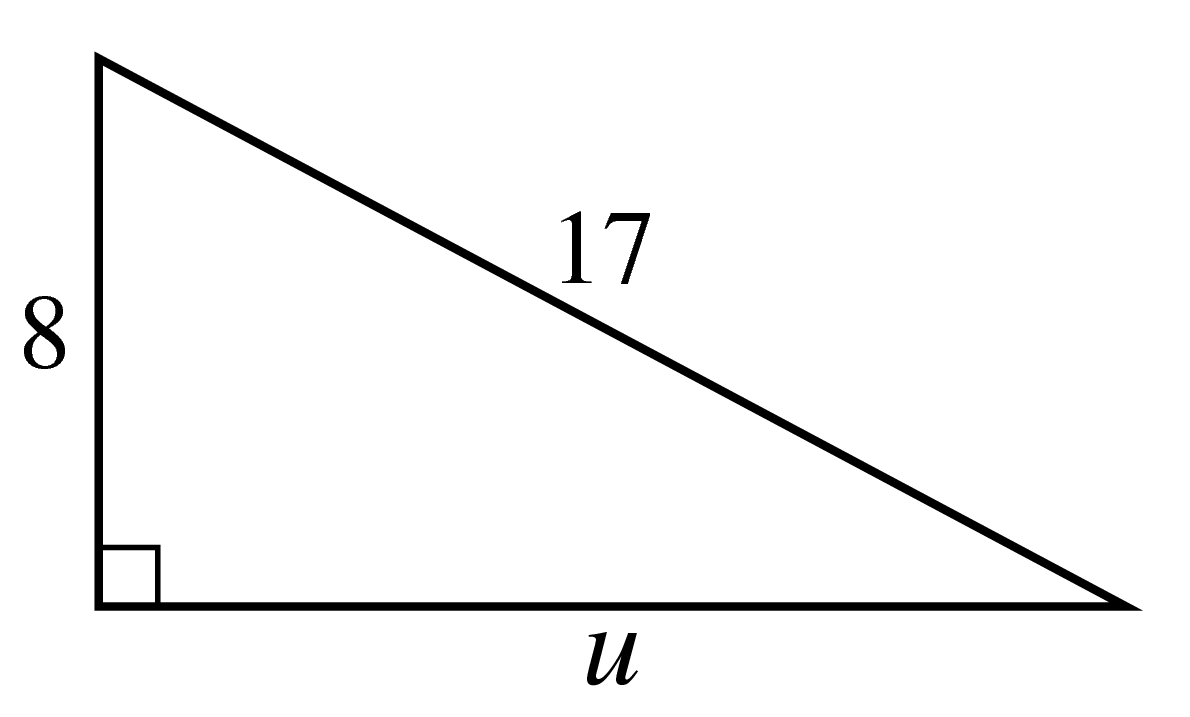
\includegraphics[width=0.85\textwidth]{images/d3.png}
    	\end{center}

    	\zs	

    		\onslide<2->{Right triangle $\Rightarrow$ Pythag.\ Thm:
    		
    		 			\zs \zs
    		
    		    		\begin{equation*}
    		    			    		a^2 +b^2 = c^2
    		    		\end{equation*}}

	  	\end{column}
    
    
    				%%% Column Break %%%
    
    
    	\begin{column}{0.5\textwidth}
    		\begin{exampleblock}{}
    			Solve for the value of $u$.
    		\end{exampleblock}

    			\zs \zs

    			\begin{align*}
    				\onslide<3->{  8^2 + u^2   &=   17^2  } \\
    				\onslide<4->{  64 + u^2   &=   289  } \\
    				\onslide<5->{  u^2   &=   225  } \\
    				\onslide<6->{  u   &=   \sqrt{225}  } \\
    				\onslide<7->{  u   &=   \sqrt{15^2}  } \\
    				\onslide<8->{  u   &=   \answerbox<9->{15}  }
    			\end{align*}


    	\end{column}
    
    \end{columns}
	

\end{frame}




%%%%%%%%%%%%%%% FRAME BREAK %%%%%%%%%%%%%%%




\begin{frame}\frametitle{\# 3}

    		\begin{exampleblock}{}
    			Which of the below are right triangles?
    		\end{exampleblock}

    			\zs
    
	\begin{columns}
	
		\begin{column}{0.5\textwidth}
			\begin{center}
				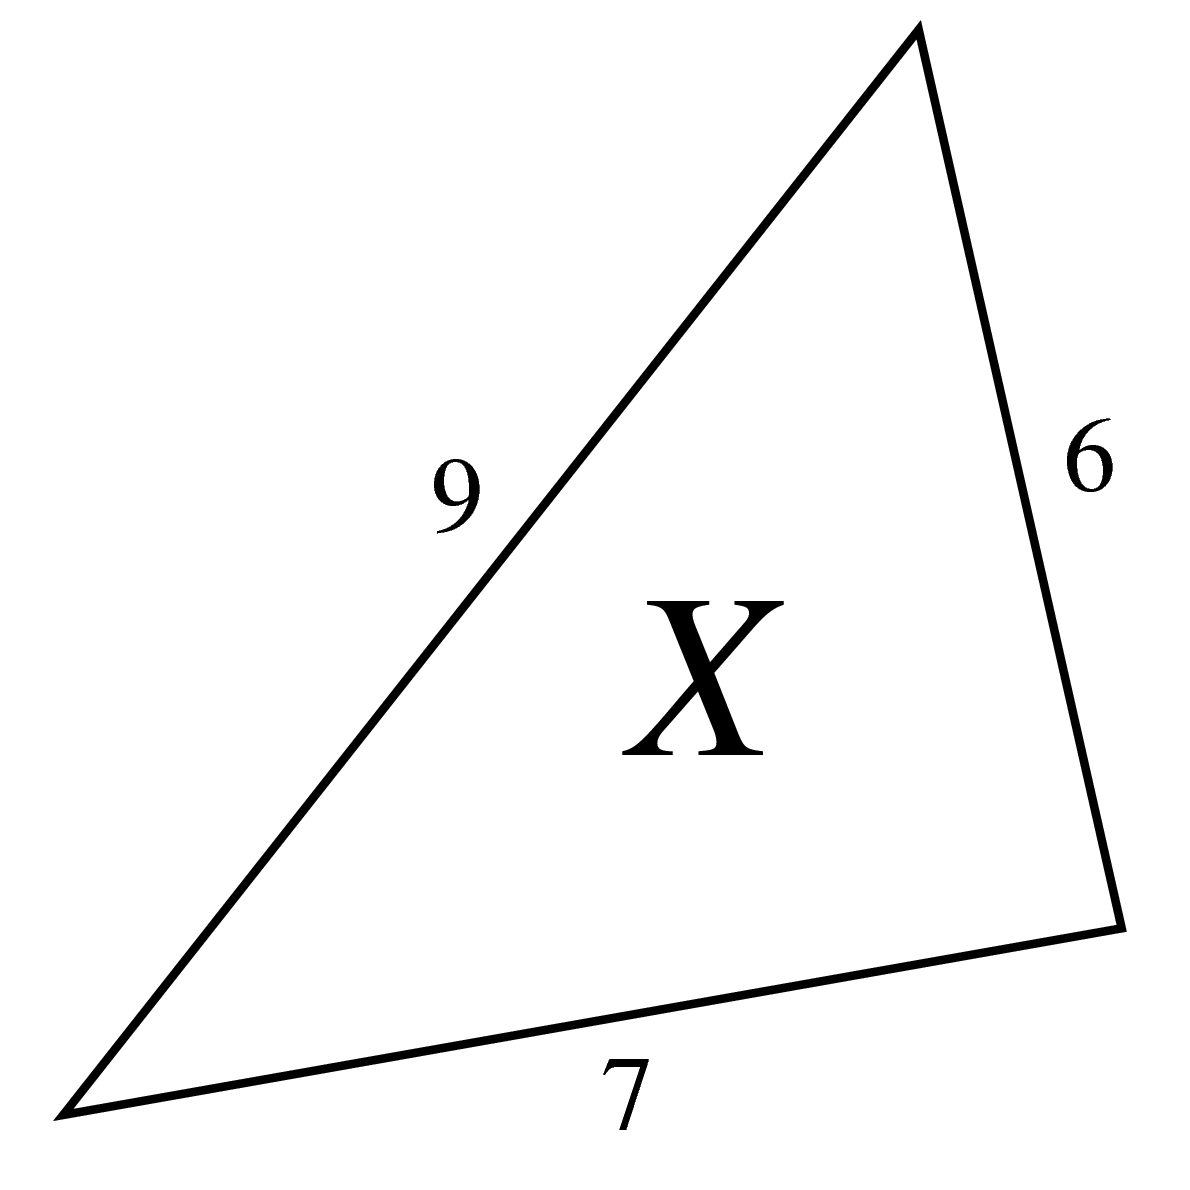
\includegraphics[width=0.7\textwidth]{images/d4.png}
			\end{center}
		\end{column}
	
	
					%%% Column Break %%%
	
	
		\begin{column}{0.5\textwidth}
			\begin{center}
				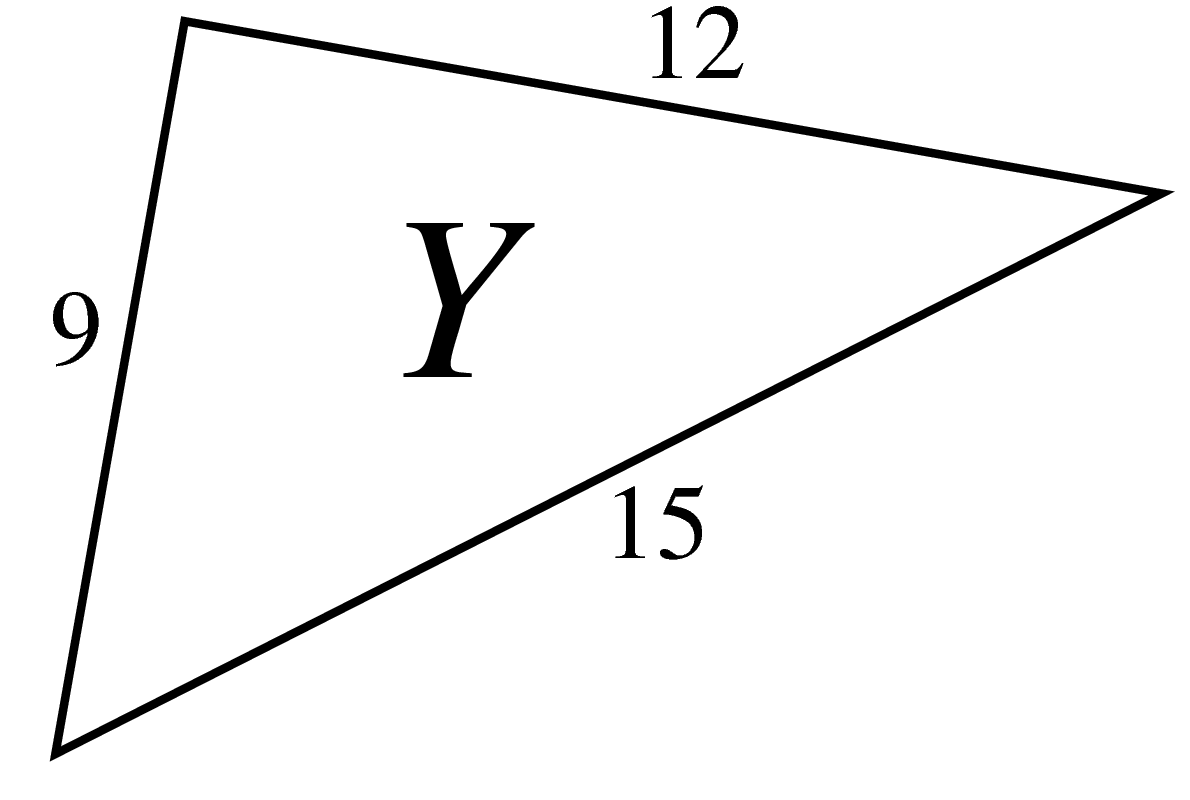
\includegraphics[width=0.7\textwidth]{images/d5.png}
			\end{center}
		\end{column}
	
	\end{columns}
	\pause \bs

	\textbf{\underline{If:}} $a^2 + b^2 = c^2$; \quad \underline{\textbf{Then:}} Right triangle\qquad \pause{\footnotesize(where $c$ is longest side)}

\end{frame}





%%%%%%%%%%%%%%% FRAME BREAK %%%%%%%%%%%%%%%




\begin{frame}\frametitle{\# 3, cont.}

			\fbox{\textbf{\underline{If:}} $a^2 + b^2 = c^2$; \quad \underline{\textbf{Then:}} Right triangle}

			\bs
    
	\begin{columns}
	
		\begin{column}{0.4\textwidth}
			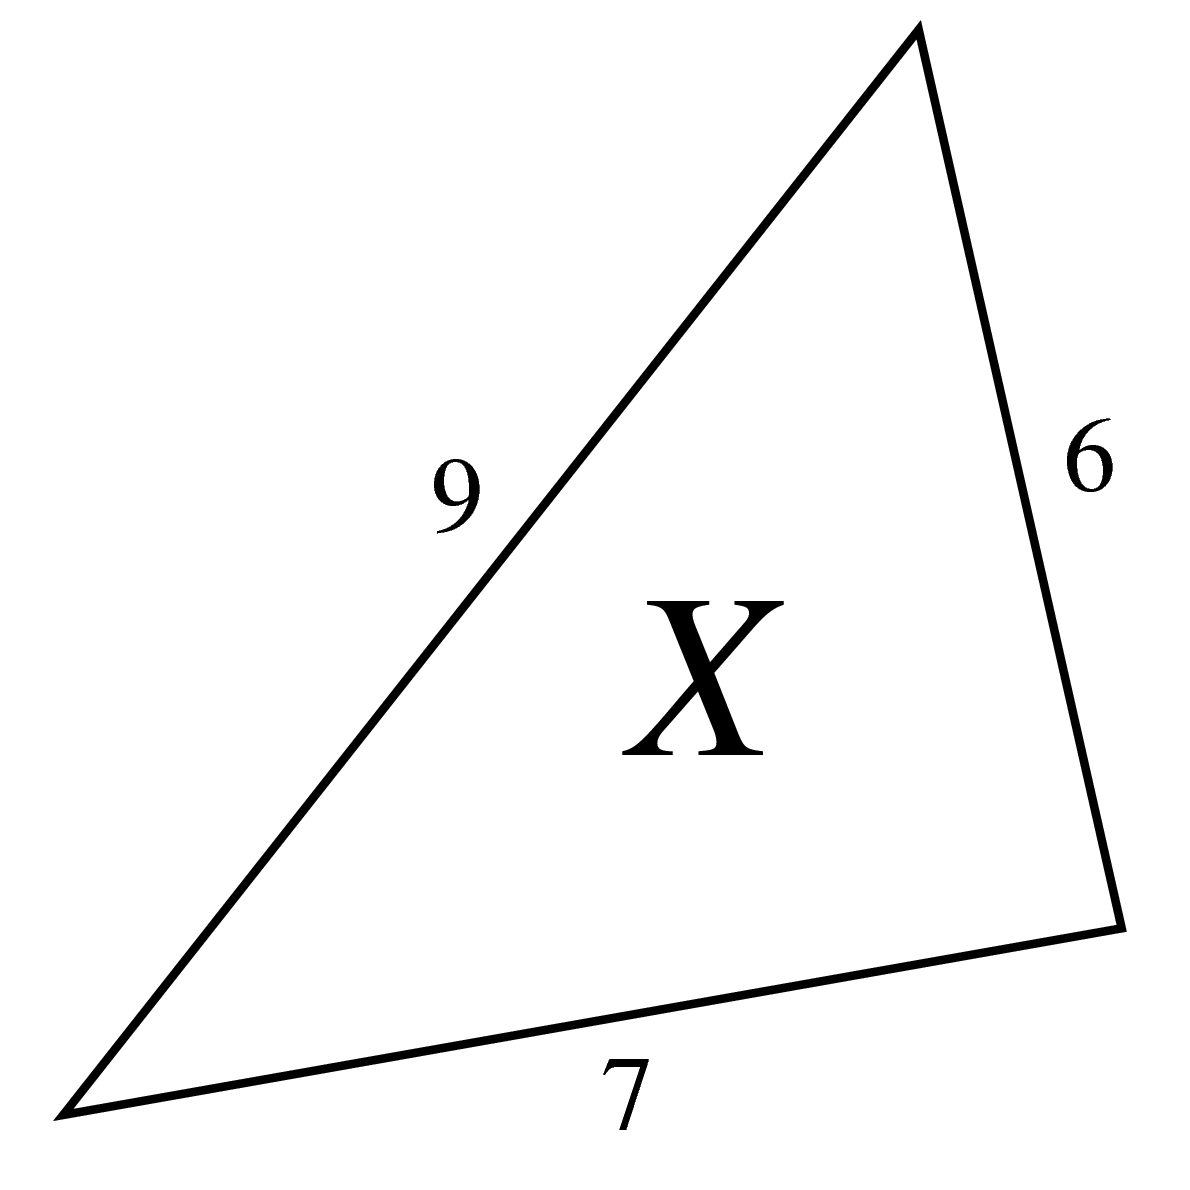
\includegraphics[width=\textwidth]{images/d4.png}
		\end{column}
	
	
					%%% Column Break %%%
	
	
		\begin{column}{0.6\textwidth}
			\begin{align*}
				\onslide<2->{  7^2 + 6^2   &\?   9^2  } \\
				\onslide<3->{  49 + 36   &\?   81  } \\
				\onslide<4->{  85   &\alert{\neq}   81  }
			\end{align*}

			\onslide<5->{\answerbox<5>{$X$ is \textbf{not} a right triangle.}}

			\bs

			\onslide<6->{($85 \alert{>} 81 \Rightarrow$ $X$ is an \emph{\textbf{acute}} triangle.)}
		\end{column}
	
	\end{columns}

\end{frame}





%%%%%%%%%%%%%%% FRAME BREAK %%%%%%%%%%%%%%%




\begin{frame}\frametitle{\# 3, cont.}
    
	\vspace{1cm}
    
	\begin{columns}
	
		\begin{column}{0.4\textwidth}
			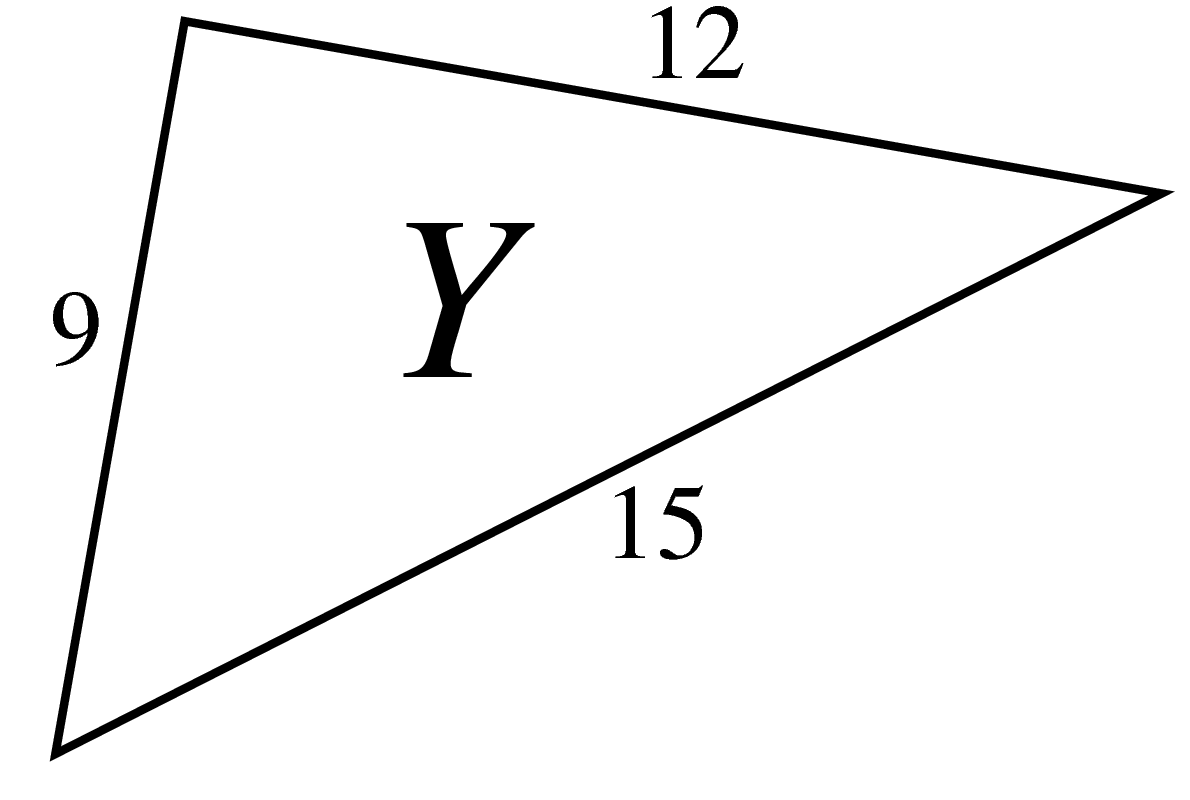
\includegraphics[width=\textwidth]{images/d5.png}
		\end{column}
	
	
					%%% Column Break %%%
	
	
		\begin{column}{0.6\textwidth}
			\begin{align*}
				\onslide<1->{  a^2 +b^2   &\?   c^2  } \\			
				\onslide<2->{  12^2 + 9^2   &\?   15^2  } \\
				\onslide<3->{  144 + 81   &\?   225  } \\
				\onslide<4->{  225   &\alert{=}   225  }
			\end{align*}

			\onslide<5->{\answerbox{$Y$ \textbf{is} a right triangle.}}
		\end{column}
	
	\end{columns}

\end{frame}




%%%%%%%%%%%%%%% FRAME BREAK %%%%%%%%%%%%%%%




\begin{frame}\frametitle{\# 4}
    
	\begin{columns}
	
		\begin{column}{0.27\textwidth}
			\as

			\includegraphics<1-2,5->[width=\textwidth]{images/d6.png}
			\includegraphics<3-4>[width=\textwidth]{images/d7.png}
		\end{column}

		\begin{column}{0.05\textwidth}
				% Space filling column
			\end{column}
	
	
					%%% Column Break %%%
	
	
		\begin{column}{0.6\textwidth}
			\begin{exampleblock}{}
				Solve for $x$.
			\end{exampleblock}

				\zs \zs \zs

			\begin{align*}
				\onslide<2->{  \textcolor<3>{Blue}{a}^2 + b^2   &=   \textcolor<3>{Red}{c}^2  } \\
				\onslide<4->{  (\textcolor<4>{Blue}{x-3})^2 + 12^2   &=   (\textcolor<4>{Red}{x+5})^2  }\\
				\onslide<5->{ (x-3)(x-3) + 144 &= (x+5)(x+5) }\\
				\onslide<6->{ \textcolor<7>{IndianRed}{x^2} -6x + 9 + 144 &= \textcolor<7>{IndianRed}{x^2} + 10x + 25 }\\
				\onslide<8->{ -6x + 153 &= 10x + 25 }\\
				\onslide<9->{ 128 &= 16x }\\
				\onslide<10->{ \answerbox<11->{8}  &= x }
			\end{align*}
		\end{column}
	
	\end{columns}

\end{frame}




%%%%%%%%%%%%%%% FRAME BREAK %%%%%%%%%%%%%%%




\begin{frame}\frametitle{\# 5}
    
	\begin{columns}
	
		\begin{column}{0.4\textwidth}
			\includegraphics<1-2>[width=\textwidth]{images/d8.png}
			\includegraphics<3>[width=\textwidth]{images/d9.png}
			\includegraphics<4>[width=\textwidth]{images/d10.png}
			\includegraphics<5->[width=\textwidth]{images/d11.png}
		\end{column}
	
	
					%%% Column Break %%%
	
	
		\begin{column}{0.6\textwidth}
			\begin{exampleblock}{}
				How long is the \alert<2>{square}'s diagonal?
			\end{exampleblock}

			\zs \zs

			\begin{align*}
				\onslide<6->{  5^2 + 5^2   &=   d^2  } \\
				\onslide<7->{  25 + 25   &=   d^2  } \\
				\onslide<8->{  50   &=   d^2  } \\
				\onslide<9->{  \sqrt{50}   &=   d  } \\
				\onslide<10->{  \sqrt{25 \cdot 2}   &=   d  } \\
				\onslide<11->{  \answerbox<12->{5 \sqrt{2}}   &=   d  } 
			\end{align*}
		\end{column}
	
	\end{columns}

\end{frame}




%%%%%%%%%%%%%%% FRAME BREAK %%%%%%%%%%%%%%%




\begin{frame}\frametitle{\# 6}
    
	\begin{columns}
	
		\begin{column}{0.5\textwidth}
		\begin{exampleblock}{}
			Tom is painting a building. He has a ladder that's $4\si{\m}$ long. To do the painting, the top of the ladder must be at least $3.5 \si{\m}$ up the wall. What is the farthest that the bottom of the ladder can be from the wall?
		\end{exampleblock}
		\end{column}
	
	
					%%% Column Break %%%
	
	
		\begin{column}{0.5\textwidth}

			\begin{overlayarea}{\textwidth}{6.5cm}
			\includegraphics<2>[width=\textwidth]{images/d12.png}
						\includegraphics<3>[width=\textwidth]{images/d13.png}
						\includegraphics<4>[width=\textwidth]{images/d13-z.png}
						\includegraphics<5>[width=\textwidth]{animations/a1-ladderdown/a1-ladderdown_119.png}
						\includegraphics<6>[width=\textwidth]{animations/a2-ladderup/a2-ladderup_59.png}
			\end{overlayarea}
		\end{column}
	
	\end{columns}

\end{frame}




%%%%%%%%%%%%%%% FRAME BREAK %%%%%%%%%%%%%%%




\begin{frame}\frametitle{\# 6, cont.}
    
	\begin{columns}
	
		\begin{column}{0.5\textwidth}
			\includegraphics<1>[width=\textwidth]{images/d14.png}
			\includegraphics<2>[width=\textwidth]{images/d15.png}
			\includegraphics<3->[width=\textwidth]{images/d16.png}
		\end{column}
	
	
					%%% Column Break %%%
	
	
		\begin{column}{0.5\textwidth}
			\begin{align*}
				\onslide<4->{  3.5^2 + x^2   &=   4^2  } \\
				\onslide<5->{  12.25 + x^2   &=   16  } \\
				\onslide<6->{  x^2   &=   3.75  } \\
				\onslide<7->{  x   &=   \sqrt{3.75} \onslide<8->{\approx 1.93649}  } \\
				\onslide<9->{  x   &=   \answerbox<10->{1.94 \onslide<10->{\si{\m}}}  } 
			\end{align*}
		\end{column}
	
	\end{columns}

\end{frame}


%%%%%%%%%%%%%%% FRAME BREAK %%%%%%%%%%%%%%%

%%% Lesson finished, Ending Slide %%%


	% Future note: While this boilerplate ending slide looks pretty decent, it could be improved upon. A good thing to do would be to create a static image in photoshop, then just re-use that. This will do for the pilot though.


\begin{frame}[b]\frametitle{Thanks for Watching!}
    
\vspace{0.25cm}

				%%% Column Break %%%




		\begin{center}
			\large Watch the rest of the videos on this topic!
			\vspace{0.1cm}

			\LARGE
			\underline{www.\Huge\textbf{chipmunkmath}\LARGE.com} \normalsize

			\bigskip


		\end{center}




\vspace{0cm}


\begin{columns}[c]

	\begin{column}{0.45\textwidth}

	\vspace{0.5cm}

		\quad \! \LARGE\textcolor[RGB]{85,172,238}{\faTwitter}\large \raisebox{0.27em}{@ChipmunkMath}\normalsize



	\end{column}


				%%% Column Break %%%

				\begin{column}{0.05\textwidth}
					\vspace{0.1cm}
					\begin{center}
						\rule{0.03cm}{2.6cm}
					\end{center}
				\end{column}


	\begin{column}{0.5\textwidth}
		\begin{center}
		\fbox{\,\includegraphics<1->[width=0.08\textwidth]{../../chipmunk-transparent.png} \,\,\, \small \raisebox{0.25em}{\textcolor<1->{Crimson}{\faHeart} \,\,\,Free Education}\,}
		\end{center}
		\vspace{-0.3cm}
		
		
		\small Creative Commons: \, \scriptsize \ccLogo \, \ccAttribution \, \ccNonCommercial \, \ccShareAlike \small

		Open source, available on GitHub \normalsize \faGithub \small

		Details at chipmunkmath.com

	\end{column}

\end{columns}


\end{frame}





\end{document}